\section{Introduction}
\label{sec:unsupervised_intro}
This work was presented at the IEEE International Symposium on Biomedical Imaging 2021 and published as part of its proceedings \citep{carse2021unsupervised}.

\subsection{Unsupervised Representation Learning for Images}
\label{subsec:unsupervised_for_medical}
As discussed in section \ref{subsec:active_for_medical_image_analysis}, modern deep learning algorithms have been shown to improve digital pathology tasks such as nuclei detection and disease classification~\citep{litjens2017survey}. They have been able to achieve such results by jointly learning deep representations and discriminative classifiers or regressors. This end-to-end training allows them to learn feature representations tailored to a given task. However, this approach requires more annotated data than traditional machine learning methods to obtain good generalization. This need for large, annotated datasets has been identified as a key challenge for digital pathology~\citep{madabhushi2016image}, as well as other medical image analysis domains. To tackle this challenge we previously experiment with active learning (Chapter \ref{ch:active_learning}) and after finding the results limiting in Section \ref{sec:active_conclusion} it was decided to focus attention on unsupervised representation learning to get the most information from unannotated images. The learnt representations from unsupervised learning can be used in multiple ways to improve generalisation, decrease data dimensionality, improve computational performance, and initialize deep supervised learning models when access to annotated data is limited~\citep{bengio2013representation}.

\begin{figure}
	\begin{minipage}[b]{.4\linewidth}
		\centering
		\centerline{\includegraphics[width=\textwidth]{images/cat.jpg}}
		\centerline{(a)}\medskip
	\end{minipage}
	\hfill
	\begin{minipage}[b]{0.4\linewidth}
		\centering
		\centerline{\includegraphics[width=\textwidth]{images/cat_grid_v2.png}}
		\centerline{(b)}\medskip
	\end{minipage}
	\\
	\begin{minipage}[b]{.4\linewidth}
		\centering
		\centerline{\includegraphics[width=\textwidth]{images/histo.png}}
		\centerline{(c)}\medskip
	\end{minipage}
	\hfill
	\begin{minipage}[b]{.4\linewidth}
		\centering
		\centerline{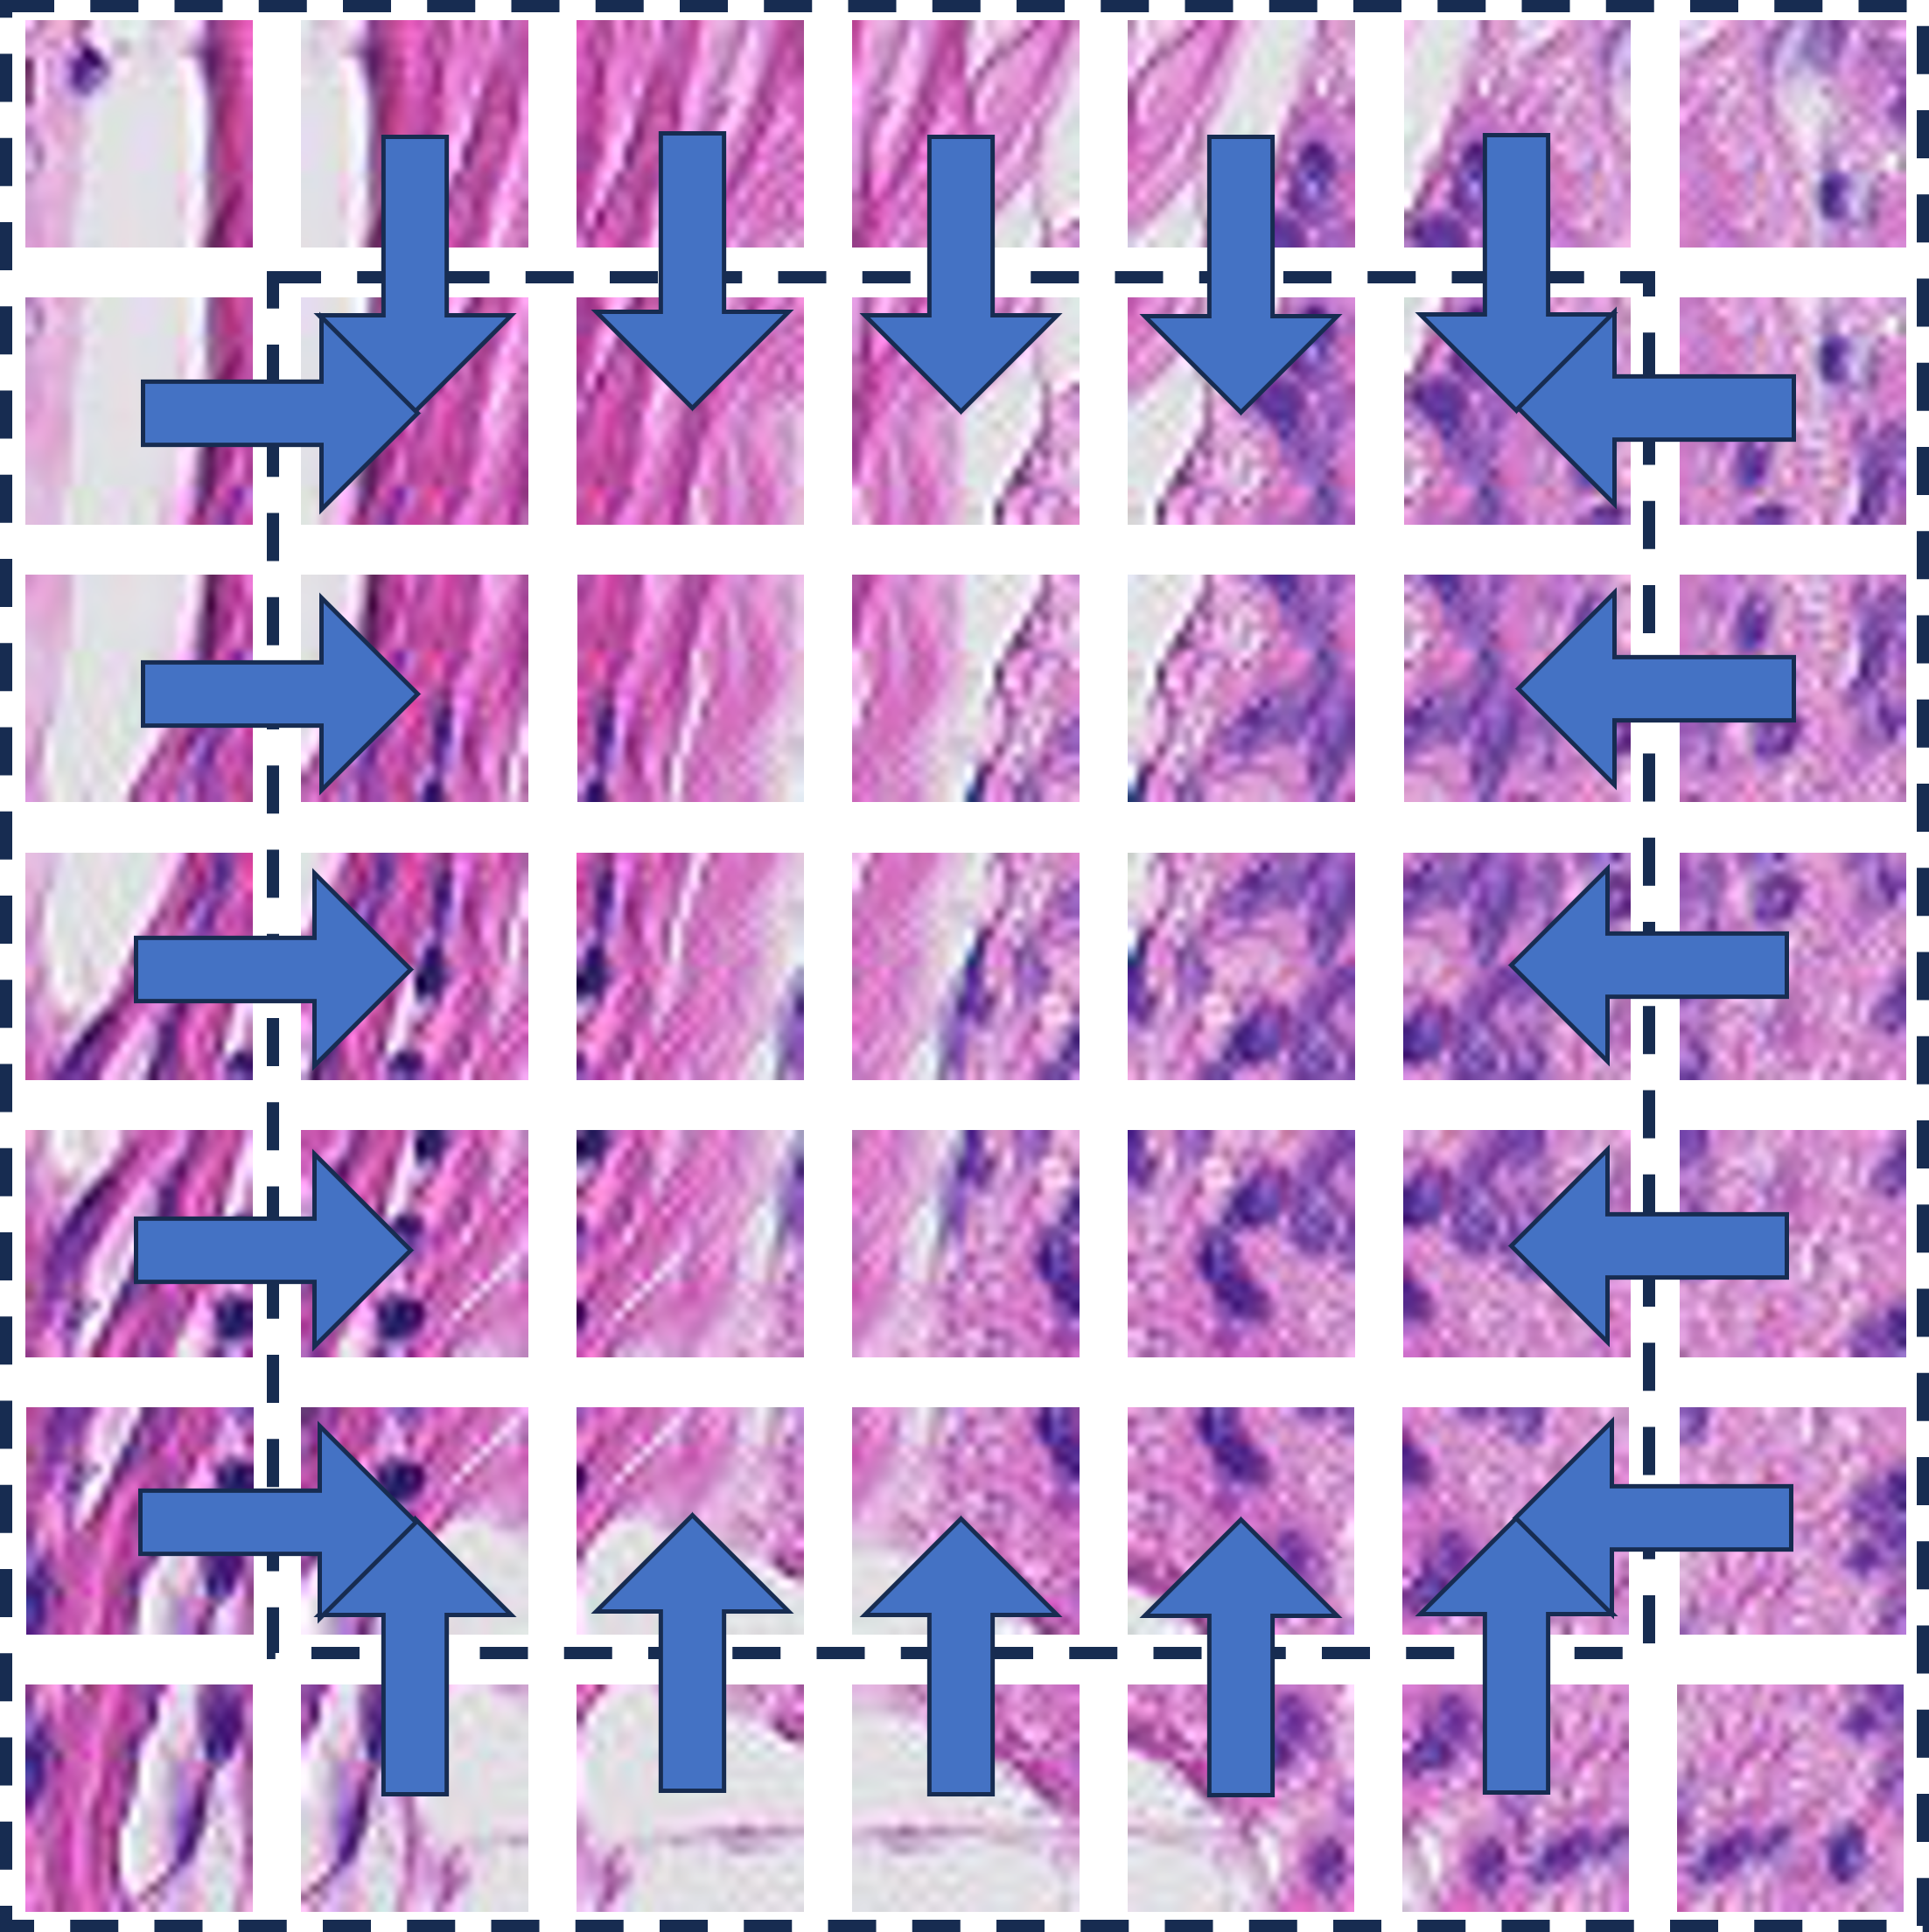
\includegraphics[width=\textwidth]{images/histo_grid.png}}
		\centerline{(d)}\medskip
	\end{minipage}
	\caption{(a) An example image from the ImageNet dataset~\cite{deng2009imagenet}. (b) Extracted overlapping patches with those used to produce context and autoregressor direction highlighted. (c) An example image from the Patch Camelyon dataset~\cite{veeling2018rotation}. (d) Extracted overlapping patches with those used to produce context and autoregressor direction highlighted.}
	\label{fig:example_cpc_patches}
\end{figure}

Transfer learning is performed by using the weights of a deep encoder used for generating representations to initialise another model~\citep{weiss2016survey}. Such an approach can reduce the need for large, annotated datasets as the model is initialised with parameters that can produce domain-representative features, having already been trained on a large pool of unannotated data. Contrastive predictive coding (CPC) is a state-of-the-art method for unsupervised representation learning~\citep{oord2018representation}. It learns data representations using an autoregressive model to predict future data representations in a sequence. A CPC model is trained using a loss function composed of two parts, a noise-contrastive estimation and importance sampling where the density ration between each sample and their representation can be preserved by classifying a positive sample and their representation can be preserved by classifying a positive sample from multiple negative samples. While this method was originally developed for sequential data (such as text) the authors purposed a method to apply CPC to images by splitting each image into overlapping patches and use an encoder to encode each patch to produce a matrix of feature representations. A mask is then applied to this matrix so that to an autoregressive model only see the top few rows of the matrix are visible. The autoregressive model is then used to predict the representations of the masked patches from the context available to it. An example of this framework being applied to an image can be seen in Figure~\ref{fig:example_cpc_patches}(b).

CPC has been used to achieve data-efficient results for object detection and Imagenet classification tasks after modifying model capacity, introducing layer normalization, modifying prediction directions, and adding patch-based augmentations~\citep{henaff2019data}. Although the autoregressive model’s predictions were made in multiple directions these were done individually. This can be an inefficient approach when dealing with images where the orientation of the image is arbitrary and does not carry useful information. This is the case for many (though not all) digital pathology tasks, in contrast to images in typical computer vision tasks.

\subsection{Summary of Work}
\label{subsec:unsupervised_summary}
This work was based on the notion that using unsupervised representation learning to learn deep representations and then using transfer learning before starting the process of active learning to learn a discriminative classifier with limited data annotations needed (Figure~\ref{fig:active_unsupervised_learning_framework}). This would remove the need for complex deep learning specific active learning query strategies and instead can focus on uncertainty-based querying. Before this, a state-of-the-art unsupervised representation learning algorithm for digital pathology images was needed. This led to the proposal of the multi-directional CPC extension with an alternative mask for building latent context and a new extension to the autoregressive model PixelCNN~\citep{oord2016pixel} for multi-directional predictions (Figure~\ref{fig:example_cpc_patches}(d)). The modification was demonstrated using the PatchCamelyon dataset~\citep{veeling2018rotation} (derived from the Camelyon16 dataset~\citep{litjens20181399}), that classification can be performed with less annotated data using representations learned in this way.

\begin{figure}
	\centering
	\includegraphics[width=\textwidth]{images/active_unsupervised_learning.png}
	\caption{Proposed active learning framework with learnt representations from unsupervised representation learning on unannotated data.}
	\label{fig:active_unsupervised_learning_framework}
\end{figure}



\section{Review of Deep Unsupervised Representation Learning}
\label{sec:unsupervised_review}
Review of Deep Unsupervised Representation Learning

\subsection{Unsupervised Representation Learning}
\label{subsec:unsupervised_representation}
Unsupervised Representation Learning

\subsection{Deep Unsupervised Representation Learning}
\label{subsec:unsupervised_deep_representation}
Deep Unsupervised Representation Learning

\subsection{Unsupervised Representation Learning for Medical Images}
\label{subsec:unsupervise_representation_for_medical}
Unsupervised Representation Learning for Medical Images



\section{Multi-Directional Contrastive Predictive Coding}
\label{sec:unsupervised_multi_directional_cpc}
Multi-Directional Contrastive Predictive Coding

\subsection{Contrastive Predictive Coding}
\label{subsec:unsupervised_cpc}
Contrastive predictive coding is a method to learn feature representations in an unsupervised manner from sequential data. A CPC model is trained by predicting future representations from past representations, enabling the model to learn ‘slow’ features that effectively represent an input data distribution~\citep{henaff2019data,oord2018representation}. A CPC model is made up of two components, the first is an encoder $g_{en}$ that encoders each element, $x_t$ of the input sequence $x$ into a latent representation $z_t = g_{en}(x_t)$. The second component is an autoregressive model $g_{ar}$, that summarises part of the latent representation sequence $z_{\le t}$ into a latent context representation $c_t = g_{ar}(z_{\le t})$. Rather than using the autoregressive model to predict future samples, a density ratio is modelled instead that preserves the mutual information between $x_{t+k}$ and $c_t$ (Equation~\ref{eq:density_ratio}).

\begin{equation}
	f_k(x_{t+k}, c_t) \propto \frac{p(x_{t+k}|c_t)}{p(x_{t+k})}
	\label{eq:density_ratio}
\end{equation}

There is no way to evaluate $p(x)$ or $p(x|c)$ directly, but as the distribution can be sampled, Noise-contrastive estimation~\citep{gutmann2010noise} can be used by comparing target value to random negative samples. The loss function used to jointly optimise the encoder and autoregressive models are dubbed InfoNCE (Equation~\ref{eq:InfoNCE}) and is based on Noise-contrastive estimation. This loss function using a set $X=\{x_i,…,x_N\}$ of $N$ random samples containing one positive sample from $p(x_{t+k}|c_t)$ and $N – 1$ negative samples from $p(x_{t+k})$. By optimising this loss the result will be $f_k(x_{t+k}, c_t)$ that estimates the density ratio from Equation~\ref{eq:density_ratio}.

\begin{equation}
	L=-\underset{x}{\mathbb{E}}\left[\log\frac{f_k(x_{t+k},c_t)}{\sum_{x_j\in X}f_k(x_j,c_t))}\right]
	\label{eq:InfoNCE}
\end{equation} 

\subsection{Contrastive Predictive Coding for Computer Vision}
\label{subsec:unsupervised_cpc_for_vision}
Contrastive Predictive Coding was originally purposed for sequential data and has been applied to computer vision by first splitting an input image into overlapping patches. Each of these patches is then encoded and an autoregressive model is used to produce a context vector from the patch representations at the top of the image (as illustrated in Figure~\ref{fig:example_cpc_patches}(b) where the top 3 rows of patches were used~\citep{oord2018representation}) Each column of the image is then treated as a sequence with the context vector from the top of the image used to model the density ratio with patch representations below. CPC has been used to achieve data-efficient results on high-level computer vision datasets such as Imagenet in the study from \cite{deng2009imagenet}.

\subsection{Multi-Directional Contrastive Predictive Coding}
\label{subsec:unsupervised_mdcpc}
The treatment of columns of the representation matrix as individual sequences (as described in Section~\ref{subsec:unsupervised_cpc_for_vision}). Can negatively impact performance when working with images where image orientation is irrelevant such as histology patches or dermoscopic skin lesion images. While the orientation of certain histology whole slide images can be biologically meaningful, the orientation of image patches such as those shown in Figure~\ref{fig:fig:example_cpc_patches}(c) (sentinel lymph node) orientation is not important. In such cases, the autoregressive model can struggle to predict patch representation from the provided context as the vertical image axis is arbitrary, unlike Imagenet where it correlates with the direction of gravity acting upon the image content. This work proposes two modifications inspired by image in-filling to address this limitation: an alternative latent mask for producing a context vector, and a modified PixelCNN~\citep{oord2016pixel} for multi-directional context building. The proposed multi-directional CPC utilises these two modifications to more effectively learn representations from images where image rotation is uninformative.

\begin{figure}
	\centering
	\includegraphics[width=0.9\textwidth]{mcb.png}
	\caption{Architecture of a Multi-Directional Masked Block}
	\label{fig:multi-directional_masked_block}
\end{figure}

The modified version of the PixelCNN is used as the autoregressive model in a multi-directional CPC model. This modification replaces each masked convolutional block of the PixelCNN architecture with a multi-directional masked (Figure~\ref{fig:multi-directional_masked_block}). Each multi-directional masked block takes a single input image and by rotation 0, 90, 180 and 270 degrees produces four versions of the original image. A masked block, as described in the paper from \cite{oord2016pixel}, is then applied to each of them. The four outputs from the masked blocks are then concatenated and put through a final 1x1 convolutional layer for dimensionality reduction.

This multi-directional autoregressive model is used to learn a latent context from multiple directions at the same time. To take advantage of this we introduce an alternative latent mask inspired by in-filling. With this mask (illustrated in Figure~\ref{fig:example_cpc_patches}(d), the autoregressive model only has access to the patch representations around the perimeter of the images. The density ratio is then estimated between the context from the edges and the central patch representations. This means that images, where rotation is unimportant, can be better represented with features learned using a single directional CPC.



\section{Unsupervised Representation Learning Experiments}
\label{sec:unsupervised_experiments}
This section details the datasets, training parameters, experimental setup, and results for the experiments with multi-directional contrastive predictive coding on digital pathology whole slide patches. The code and full results used within this section can be found on the project GitHub repository\footnote{GitHub Repository: \url{github.com/UoD-CVIP/Multi_Directional_CPC_Histology}}.

\subsection{Dataset}
\label{subsec:unsupervised_dataset}
It was chosen to use the publicly available dataset Patch Cameleyon~\citep{veeling2018rotation} in our experiments. This dataset was chosen as it contains a larger number of non-overlapping whole slide image patches that have no inherent directionality for each patch and was originally used to evaluate Rotation Equivariant CNNs~\citep{veeling2018rotation}. These patches were extracted from 400 whole slide image scans of sentinel lymph node sections from the Camelyon16 dataset~\citep{litjens20181399}. These whole slide images were collected from two different centres and digitised with an objective of 40x magnification (pixel resolution of 0.243 microns). Each patch was annotated with a binary label indicating the presence or absence of metastatic tissue, by seeing if the centre 32x32 pixels of the patch contains at least one pixel of tumour. The dataset has a total of 327,680 patches and where split into training and testing with the ratio 90:10. Augmentation is also used during training by applying random rotations, random vertical and horizontal flipping as patches is being sampled.

\subsection{Experiment Setup}
\label{subsec:unsupervised_experiment}
For the experiments we conducted an ablation study by training four CPC models using different combinations of single or multi-directional autoregressive models, and top-down or in-filling style latent masks. To evaluate the learnt representations from the CPC models, the trained encoders from the CPC models are used to initialise the weights of 9 CNN classifiers. These CNN classifiers are then trained using a small, annotated subsets of the training data ranging in size from 10 to 100,000 patches on logarithmic scale, these were all tested on the same static test set. This means that for each of the 4 CPC models 9 CNN models trained and this is repeated 5 times using different subsamples from the training data. 

\subsection{Training Parameters}
\label{subsec:unsupervised_training}
To train the CPC models each input image is split into overlapping 24x24 patches overlapping each other by 12 pixels and used a ResNeXt~\citep{xie2017aggregated} with 101 layers as the encoder immediately followed by an additional convolutional layer to produce a 128-dimensional feature vector for each 24x24 patch in the image. The autoregressive model is comprised of 6 masked convolutional blocks to produce the context vector and predict the masked feature vectors. Each of the CNN models are use a ResNeXt encoder with 101 layers so that the trained parameters of the encoder from the CPC model can be used to initialise the CNN model’s encoder. This is followed by a fully connected hidden layer with 256 neurons and then a final output layer.

To train both models the gradient decent optimisation algorithm Adam~\citep{kingma2014adam} was used, with a starting learning of $1e^{-4}$. The Adam optimiser is based on adaptive estimation of first and second order moments in the parameter gradients to adjust the learning rate during training. The CPC model were trained for 20 epochs with a batch size of 16 and the CNN models were trained over 50 epochs with a batch size of 64. When training either the CPC or CNN models 20\% of the available training data is used as validation set, this means that when training the CPC model, the validation set contained 58,982 images. The validation set is used for early stopping by saving the model the when the loss is lowest on the validation set. 

For the CPC loss function 16 randomly selected images are used as negative samples, as explained in Section~\ref{subsec:unsupervised_cpc}. Each CPC model took an average of 90 hours to train using a single Nvidia GeForce RTX 2080 Ti\footnote{Nvidia RTX 20 Series: \url{www.nvidia.com/en-gb/geforce/20-series/}}. Figure~\ref{fig:cpc_training} plots the validation loss at each epoch and suggests that the use of a multi-directional autoregressive model was more efficient at reducing the InfoNCE loss than a single-directional top-down autoregressive model. The in-filling style latent mask in combination with the multi-directional autoregressive model stabilised the CPC training.

\subsection{Results}
\label{subsec:unsupervised_results}
Figure~\ref{fig:cnn_results} and Table~\ref{tab:cnn_results} show the mean accuracies on the held-out testing set (32,768 images) for CNN classifiers trained using the different CPC encoder’s weights and biases for initialisation. A baseline with CNN models that have had no pretraining was also included. The CNNs where small amounts of annotated data were used to train were able to achieve higher accuracies when a multi-directional autoregressive model is used to initialise the CNN. In contrast, standard CPC struggled to learn a representation suitable for initialising a CNN classifier, sometimes leading to lower accuracies compared to those initialises using random weights. The benefit of using the CPC pretraining decreases as the number of images increases showing that using this method of transfer learning is best suited when the number of annotated images is low.

\begin{table}[]
	\centering
	\caption{Mean test accuracies of the CNN classifiers (standard deviations in parentheses).}
	\label{tab:cnn_results}
	\resizebox{\textwidth}{!}{%
		\begin{tabular}{r|rrrrr}
			\multicolumn{1}{c|}{\begin{tabular}[c]{@{}c@{}}Training\\ Examples\end{tabular}} &
			\multicolumn{1}{c}{No Pretraining} &
			\multicolumn{1}{c}{\begin{tabular}[c]{@{}c@{}}Single-Directional\\ Normal Mask\end{tabular}} &
			\multicolumn{1}{c}{\begin{tabular}[c]{@{}c@{}}Single-Directional\\ Infilling Mask\end{tabular}} &
			\multicolumn{1}{c}{\begin{tabular}[c]{@{}c@{}}Multi-Directional\\ Normal Mask\end{tabular}} &
			\multicolumn{1}{c}{\begin{tabular}[c]{@{}c@{}}Multi-Directional\\ Infilling Mask\end{tabular}} \\ \hline
			10     & 0.518 (0.041) & 0.509 (0.029)          & 0.509 (0.055)          & \textbf{0.566 (0.071)} & 0.522 (0.045)          \\
			32     & 0.500 (0.000) & 0.520 (0.045)          & 0.551 (0.042)          & 0.573 (0.068)          & \textbf{0.614 (0.050)} \\
			100    & 0.679 (0.014) & 0.546 (0.046)          & 0.643 (0.049)          & \textbf{0.696 (0.065)} & 0.678 (0.004)          \\
			316    & 0.691 (0.053) & 0.670 (0.029)          & 0.703 (0.014)          & \textbf{0.727 (0.018)} & 0.720 (0.035)          \\
			1000   & 0.750 (0.014) & 0.713 (0.022)          & 0.731 (0.012)          & 0.747 (0.002)          & \textbf{0.769 (0.012)} \\
			3162   & 0.772 (0.017) & 0.781 (0.014)          & 0.755 (0.012)          & 0.771 (0.015)          & \textbf{0.784 (0.009)} \\
			10000  & 0.788 (0.005) & \textbf{0.798 (0.003)} & 0.797 (0.028)          & 0.788 (0.018)          & 0.778 (0.013)          \\
			31624  & 0.773 (0.003) & 0.790 (0.009)          & \textbf{0.806 (0.014)} & 0.792 (0.007)          & 0.801 (0.013)          \\
			100000 & 0.811 (0.004) & 0.802 (0.008)          & 0.804 (0.020)          & 0.805 (0.012)          & \textbf{0.816 (0.020)}
		\end{tabular}%
	}
\end{table}


\section{Conclusion}
\label{sec:conclusion}
We have shown that the original CPC architecture does not perform well on a digital pathology patch classification task. We proposed a multi-directional modification to CPC that achieved better results, and improved classification accuracies when annotated data were limited. Our experiment illustrates that algorithms based on an assumption of image directionality (such as is present in Imagenet) will not necessarily perform well on images without such directionality. We suppose that this will also be true for other visual tasks where image orientation is unimportant, as is the case in multiple biomedical imaging settings.  